\section{Contrail Detection}
\label{sec:intro}

Contrail detection is an essential component towards understanding the impact and mitigation of contrails. Being able to detect contrails with high accuracy is a necessary capability in order to evaluate and compare contrail predictive models, to track contrails through their lifespan and measure the amount of heat that they trap, and ultimately to verify the effectiveness of flight path diversion efforts.

Remote sensing satellites, equipped with state-of-the-art sensors, such as the Advanced Baseline Imager (ABI) on the Geostationary Operational Environmental Satellites (GOES) \cite{goes} have allowed for reliable and consistent environmental observations. Compared to Polar-orbiting Operational Environmental Satellites (POES) such as the Suomi or Sentinel satellites, GOES maintains constant observation over a fixed area with relatively higher temporal resolution but at the cost of lower spatial resolution. With 2 kilometer spatial resolution in the infrared bands, GOES imagery in not sufficient to caputure the initial formation of young contrails, but is able to capture the more mature stages of contrails if they continue to spread out. GOES's coarser resolution narrows our focus on the contrails with the largest climate impact since persistent contrails that have expanded sufficiently to be observable at 2 kilometer resolution are associated with more significant warming effects \cite{warm, persist}. Additionally, the proposed contrail predictive model will be at 3 kilometer resolution, thus reducing the utility of higher resolution contrail detection. 

In the last 20 years, contrails have primarily been detected in POES imagery using image processing techniques such as the Mannstein et al algorithm \cite{mannstein} that applies a series of hand engineered convolution and thresholding operations to infrared imagery. More recently, a method for tracking the lifecycle of contrails that uses the aforementioned Mannstein et al algorithm on POES imagery for early stage detection and then uses a tracking algorithm on GOES imagery for later stage contrail evolution \cite{track}. POES satellites are often contrained by a single pass per day over a given area of interest, limiting the ability to support contrail avoidance.

With the introduction of large human-labeled contrail datasets \cite{opencontrails, landsat}, more recent studies have applied deep learning based contrail detection models \cite{opencontrails, covid} with GOES imagery. While deep learning approaches have the potential to better support contrail avoidance preditions, there has not been a direct performance analysis between the Mannstein et al method and the deep learning models. Quantifying the effectiveness of contrail detection methods is crucial for accurate assessment of the cost and benefits of contrail predictive models. False positives of a high probability area for contrail formation would increase costs of fuel consumption for flights to take unecessary avoidance measures. False negatives, where a flight creates preventable contrail formations, would decrease the utility of implementing contrail predictive models. 

\begin{figure}
    \centering
    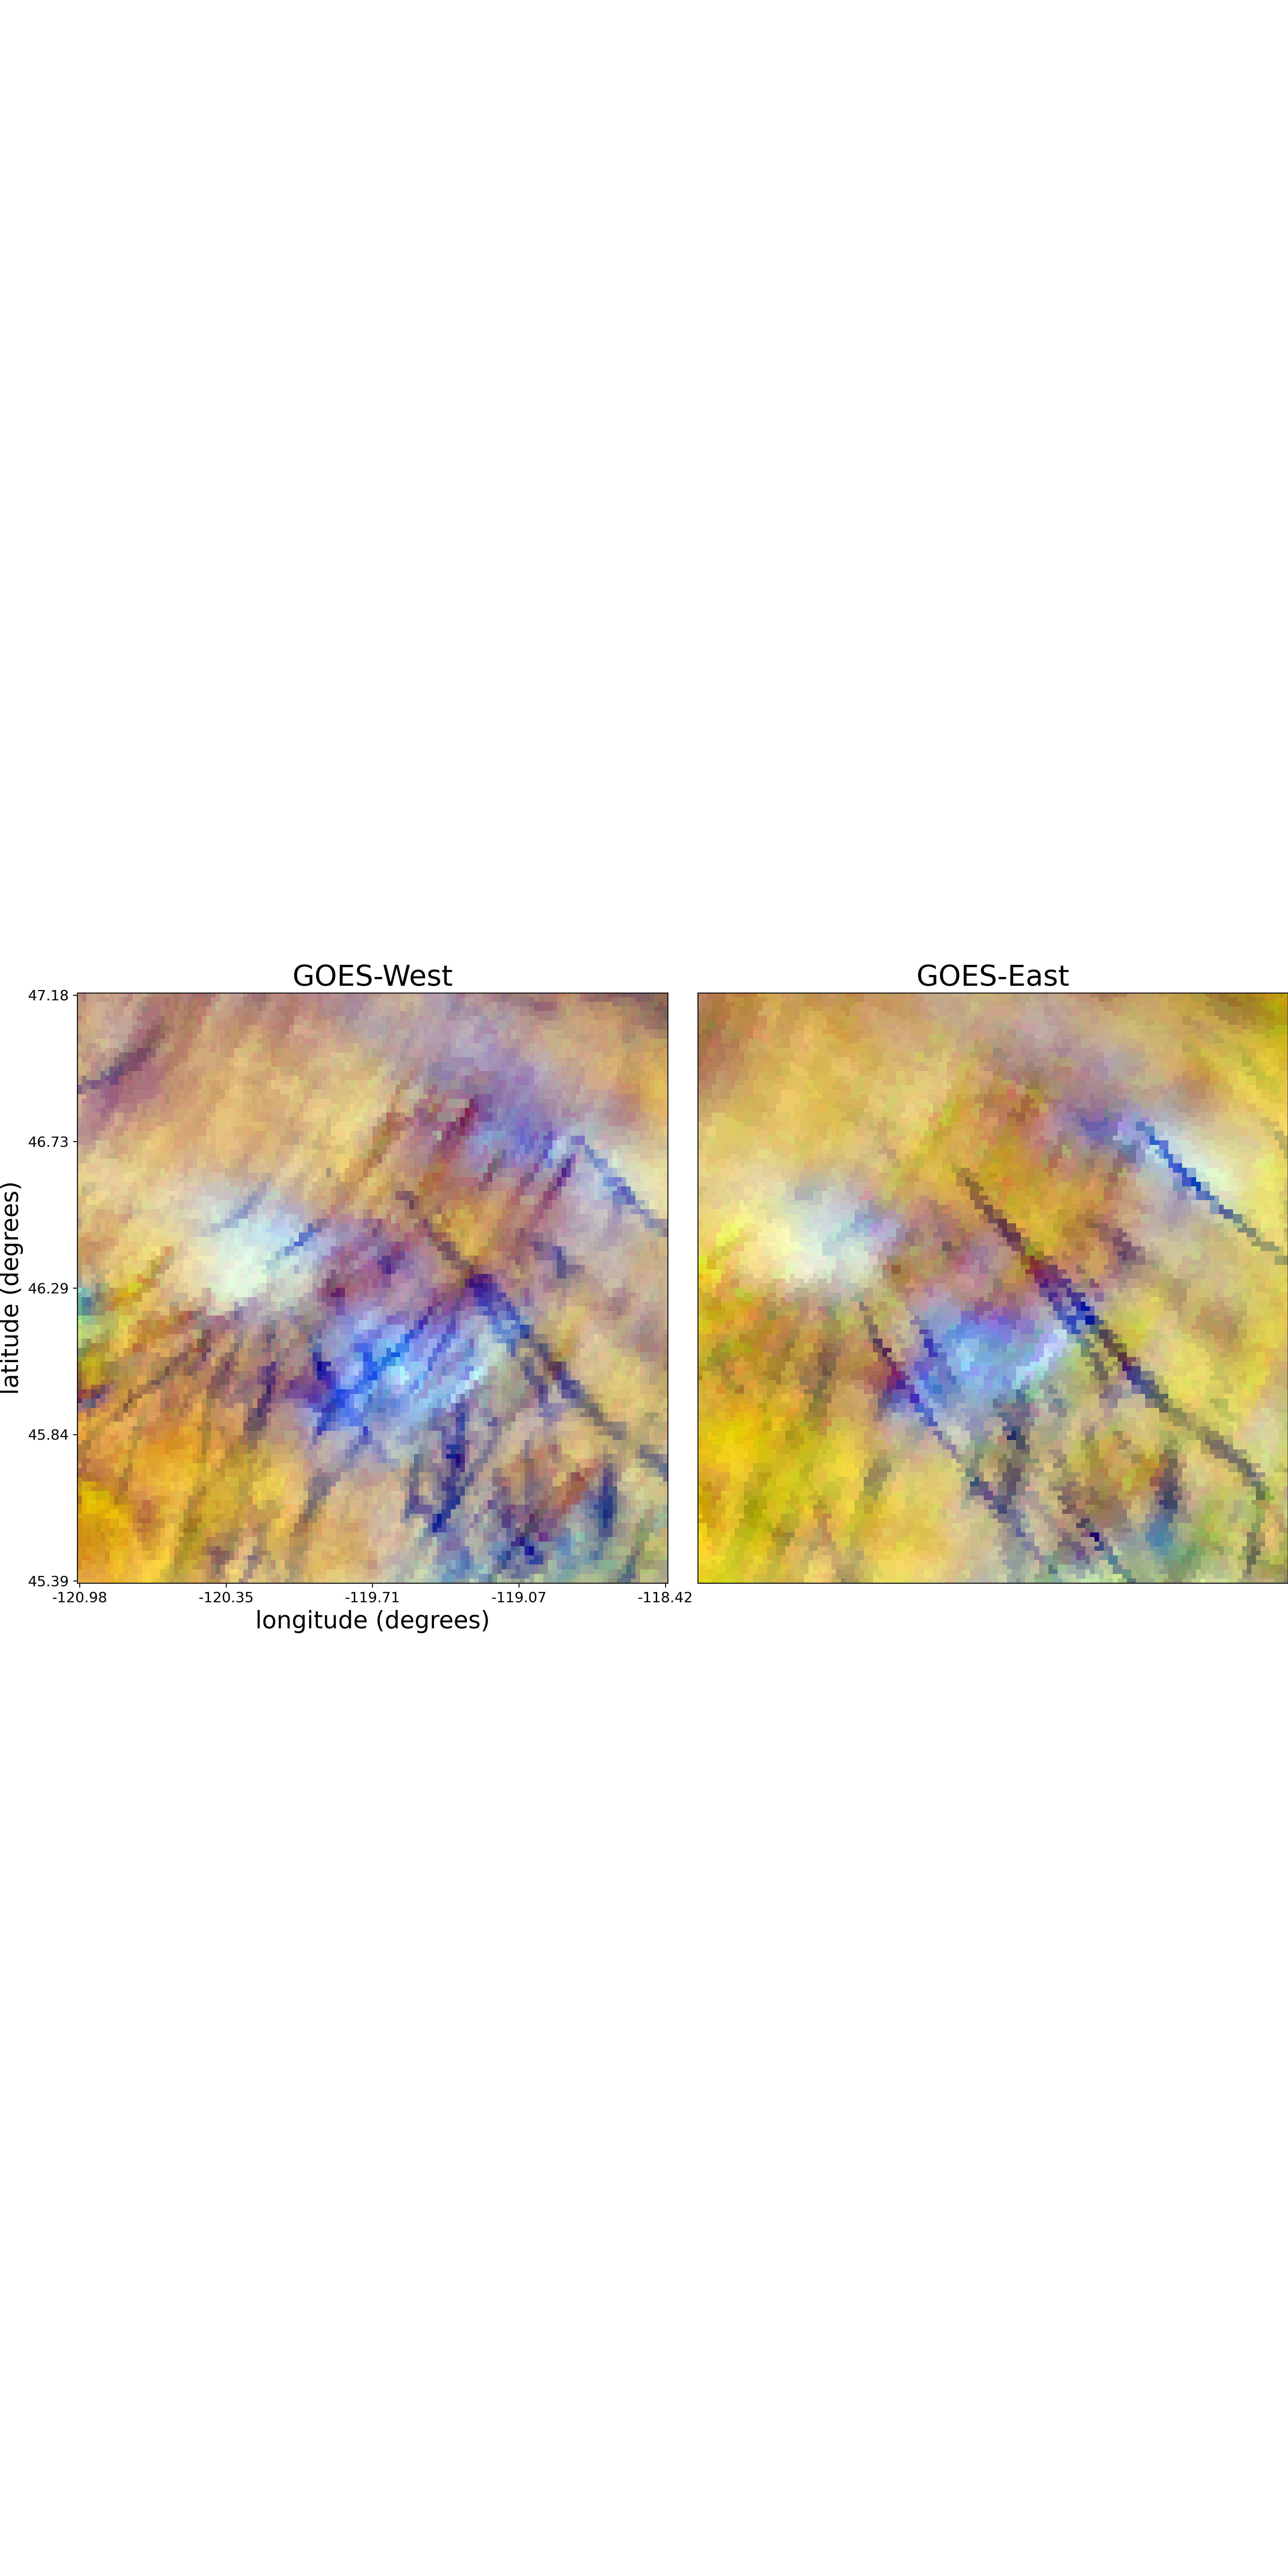
\includegraphics[width=8cm]{figures/west_best.png}
    \caption{GOES imagery from 2025/03/11 15:50 UTC using the ash composite (dark blue are cirrus), that shows that GOES-West can provide signatures of contrails that are not visible in GOES-East.}
    \label{west_best}
\end{figure}


We propose to contribute the following additions to the current literature on contrail detection:
\begin{enumerate}[label*=\arabic*.]
    \item A publicly available deep learning model trained on the GOES-East OpenContrail Dataset.
        \begin{enumerate}[label*=\arabic*.]
            \item OpenContrail did not release their models.
        \end{enumerate}
    \item An analysis of the Mannstein et al algorithm on the OpenContrail dataset.
        \begin{enumerate}[label*=\arabic*.]
            \item Compare to prior deep learning studies and our GOES-East model.
            \item This can be used to validate the deep learning models.
        \end{enumerate}
    \item A GOES-West specific contrail dataset derived from the OpenContrail dataset.
        \begin{enumerate}[label*=\arabic*.]
            \item If we apply a parallax correction to the GOES-West satellite images, we should be able to use the same human-labeled contrails made for GOES-East. 
        \end{enumerate}
    \item A deep learning model trained on the new GOES-West contrail dataset.
        \begin{enumerate}[label*=\arabic*.]
            \item GOES-East does not cover Hawaii or Alaska.
            \item Preliminary plots (figure \ref{west_best}) show that GOES-West can potentially show certain contrails missed by GOES-East.
            \item Can be used to validate the GOES-East model. 
        \end{enumerate}
    \item Altitude approximation directly from satellite imagery.
        \begin{enumerate}[label*=\arabic*.]
            \item Altitude is currently found by matching detected contrails to flight information. This is tedious and difficult to do correctly in high flight traffic areas. 
            \item We will use cloud top temperature and parallax distance to approximate flight altitude.
        \end{enumerate}

    \end{enumerate}







